\documentclass[twoside]{book}

% Packages required by doxygen
\usepackage{fixltx2e}
\usepackage{calc}
\usepackage{doxygen}
\usepackage[export]{adjustbox} % also loads graphicx
\usepackage{graphicx}
\usepackage[utf8]{inputenc}
\usepackage{makeidx}
\usepackage{multicol}
\usepackage{multirow}
\PassOptionsToPackage{warn}{textcomp}
\usepackage{textcomp}
\usepackage[nointegrals]{wasysym}
\usepackage[table]{xcolor}

% NLS support packages
\usepackage[ngerman]{babel}

% Font selection
\usepackage[T1]{fontenc}
\usepackage[scaled=.90]{helvet}
\usepackage{courier}
\usepackage{amssymb}
\usepackage{sectsty}
\renewcommand{\familydefault}{\sfdefault}
\allsectionsfont{%
  \fontseries{bc}\selectfont%
  \color{darkgray}%
}
\renewcommand{\DoxyLabelFont}{%
  \fontseries{bc}\selectfont%
  \color{darkgray}%
}
\newcommand{\+}{\discretionary{\mbox{\scriptsize$\hookleftarrow$}}{}{}}

% Page & text layout
\usepackage{geometry}
\geometry{%
  a4paper,%
  top=2.5cm,%
  bottom=2.5cm,%
  left=2.5cm,%
  right=2.5cm%
}
\tolerance=750
\hfuzz=15pt
\hbadness=750
\setlength{\emergencystretch}{15pt}
\setlength{\parindent}{0cm}
\setlength{\parskip}{3ex plus 2ex minus 2ex}
\makeatletter
\renewcommand{\paragraph}{%
  \@startsection{paragraph}{4}{0ex}{-1.0ex}{1.0ex}{%
    \normalfont\normalsize\bfseries\SS@parafont%
  }%
}
\renewcommand{\subparagraph}{%
  \@startsection{subparagraph}{5}{0ex}{-1.0ex}{1.0ex}{%
    \normalfont\normalsize\bfseries\SS@subparafont%
  }%
}
\makeatother

% Headers & footers
\usepackage{fancyhdr}
\pagestyle{fancyplain}
\fancyhead[LE]{\fancyplain{}{\bfseries\thepage}}
\fancyhead[CE]{\fancyplain{}{}}
\fancyhead[RE]{\fancyplain{}{\bfseries\leftmark}}
\fancyhead[LO]{\fancyplain{}{\bfseries\rightmark}}
\fancyhead[CO]{\fancyplain{}{}}
\fancyhead[RO]{\fancyplain{}{\bfseries\thepage}}
\fancyfoot[LE]{\fancyplain{}{}}
\fancyfoot[CE]{\fancyplain{}{}}
\fancyfoot[RE]{\fancyplain{}{\bfseries\scriptsize Erzeugt von Doxygen }}
\fancyfoot[LO]{\fancyplain{}{\bfseries\scriptsize Erzeugt von Doxygen }}
\fancyfoot[CO]{\fancyplain{}{}}
\fancyfoot[RO]{\fancyplain{}{}}
\renewcommand{\footrulewidth}{0.4pt}
\renewcommand{\chaptermark}[1]{%
  \markboth{#1}{}%
}
\renewcommand{\sectionmark}[1]{%
  \markright{\thesection\ #1}%
}

% Indices & bibliography
\usepackage{natbib}
\usepackage[titles]{tocloft}
\setcounter{tocdepth}{3}
\setcounter{secnumdepth}{5}
\makeindex

% Hyperlinks (required, but should be loaded last)
\usepackage{ifpdf}
\ifpdf
  \usepackage[pdftex,pagebackref=true]{hyperref}
\else
  \usepackage[ps2pdf,pagebackref=true]{hyperref}
\fi
\hypersetup{%
  colorlinks=true,%
  linkcolor=blue,%
  citecolor=blue,%
  unicode%
}

% Custom commands
\newcommand{\clearemptydoublepage}{%
  \newpage{\pagestyle{empty}\cleardoublepage}%
}

\usepackage{caption}
\captionsetup{labelsep=space,justification=centering,font={bf},singlelinecheck=off,skip=4pt,position=top}

%===== C O N T E N T S =====

\begin{document}

% Titlepage & ToC
\hypersetup{pageanchor=false,
             bookmarksnumbered=true,
             pdfencoding=unicode
            }
\pagenumbering{alph}
\begin{titlepage}
\vspace*{7cm}
\begin{center}%
{\Large iperf G\+UI }\\
\vspace*{1cm}
{\large Erzeugt von Doxygen 1.8.12}\\
\end{center}
\end{titlepage}
\clearemptydoublepage
\pagenumbering{roman}
\tableofcontents
\clearemptydoublepage
\pagenumbering{arabic}
\hypersetup{pageanchor=true}

%--- Begin generated contents ---
\chapter{iperf G\+UI}
\label{index}\hypertarget{index}{}Die Software iperf ist ein Kommandozeilenprogramm zum Messen der Performance und zur Netzbelastung von Netzwerken. Für dieses Programm wurde eine Grafische Benutzeroberfläche entwickelt, mit welcher auf einem Raspberry Pi mit 7“ Touch-\/\+Display die Software einfach und intuitiv bedient werden kann.

Der Haupteinsatzzweck der Software ist eine Belastung des Netzwerkes. Die Software kann gestartet und gestoppt werden und die wesentlichen Parameter, welche für eine Netzbelastung notwendig sind, können eingestellt werden. Über ein einfaches Ampelsystem wird dem Benutzer Rückmeldung gegeben. 
\chapter{Hierarchie-\/\+Verzeichnis}
\section{Class Hierarchy}
This inheritance list is sorted roughly, but not completely, alphabetically\+:\begin{DoxyCompactList}
\item Q\+Widget\begin{DoxyCompactList}
\item \contentsline{section}{Client}{\pageref{class_client}}{}
\item \contentsline{section}{Num\+Pad}{\pageref{class_num_pad}}{}
\item \contentsline{section}{Server}{\pageref{class_server}}{}
\item \contentsline{section}{Traffic\+Light}{\pageref{class_traffic_light}}{}
\item \contentsline{section}{Welcome\+Screen}{\pageref{class_welcome_screen}}{}
\end{DoxyCompactList}
\end{DoxyCompactList}

\chapter{Klassen-\/\+Verzeichnis}
\section{Auflistung der Klassen}
Hier folgt die Aufzählung aller Klassen, Strukturen, Varianten und Schnittstellen mit einer Kurzbeschreibung\+:\begin{DoxyCompactList}
\item\contentsline{section}{\hyperlink{class_client}{Client} \\*Die Client-\/\+Klasse }{\pageref{class_client}}{}
\item\contentsline{section}{\hyperlink{class_iperf_interface}{Iperf\+Interface} \\*Die Iperf\+Interface-\/\+Klasse }{\pageref{class_iperf_interface}}{}
\item\contentsline{section}{\hyperlink{class_num_pad}{Num\+Pad} \\*Die Num\+Pad-\/\+Klasse }{\pageref{class_num_pad}}{}
\item\contentsline{section}{\hyperlink{class_server}{Server} \\*Die Server-\/\+Klasse }{\pageref{class_server}}{}
\item\contentsline{section}{\hyperlink{class_traffic_light}{Traffic\+Light} \\*Die Traffic\+Light-\/\+Klasse }{\pageref{class_traffic_light}}{}
\item\contentsline{section}{\hyperlink{class_welcome_screen}{Welcome\+Screen} \\*Die Welcome\+Screen-\/\+Klasse }{\pageref{class_welcome_screen}}{}
\end{DoxyCompactList}

\chapter{Datei-\/\+Verzeichnis}
\section{File List}
Here is a list of all documented files with brief descriptions\+:\begin{DoxyCompactList}
\item\contentsline{section}{src/\hyperlink{client_8h}{client.\+h} \\*A brief description about this header file }{\pageref{client_8h}}{}
\item\contentsline{section}{src/\hyperlink{main_8cpp}{main.\+cpp} \\*The main file of this project }{\pageref{main_8cpp}}{}
\item\contentsline{section}{src/{\bfseries numpad.\+h} }{\pageref{numpad_8h}}{}
\item\contentsline{section}{src/{\bfseries server.\+h} }{\pageref{server_8h}}{}
\item\contentsline{section}{src/{\bfseries trafficlight.\+h} }{\pageref{trafficlight_8h}}{}
\item\contentsline{section}{src/{\bfseries welcomescreen.\+h} }{\pageref{welcomescreen_8h}}{}
\end{DoxyCompactList}

\chapter{Klassen-\/\+Dokumentation}
\hypertarget{class_client}{}\section{Client Klassenreferenz}
\label{class_client}\index{Client@{Client}}


Die Client-\/\+Klasse.  




{\ttfamily \#include $<$client.\+h$>$}

Klassendiagramm für Client\+:\begin{figure}[H]
\begin{center}
\leavevmode
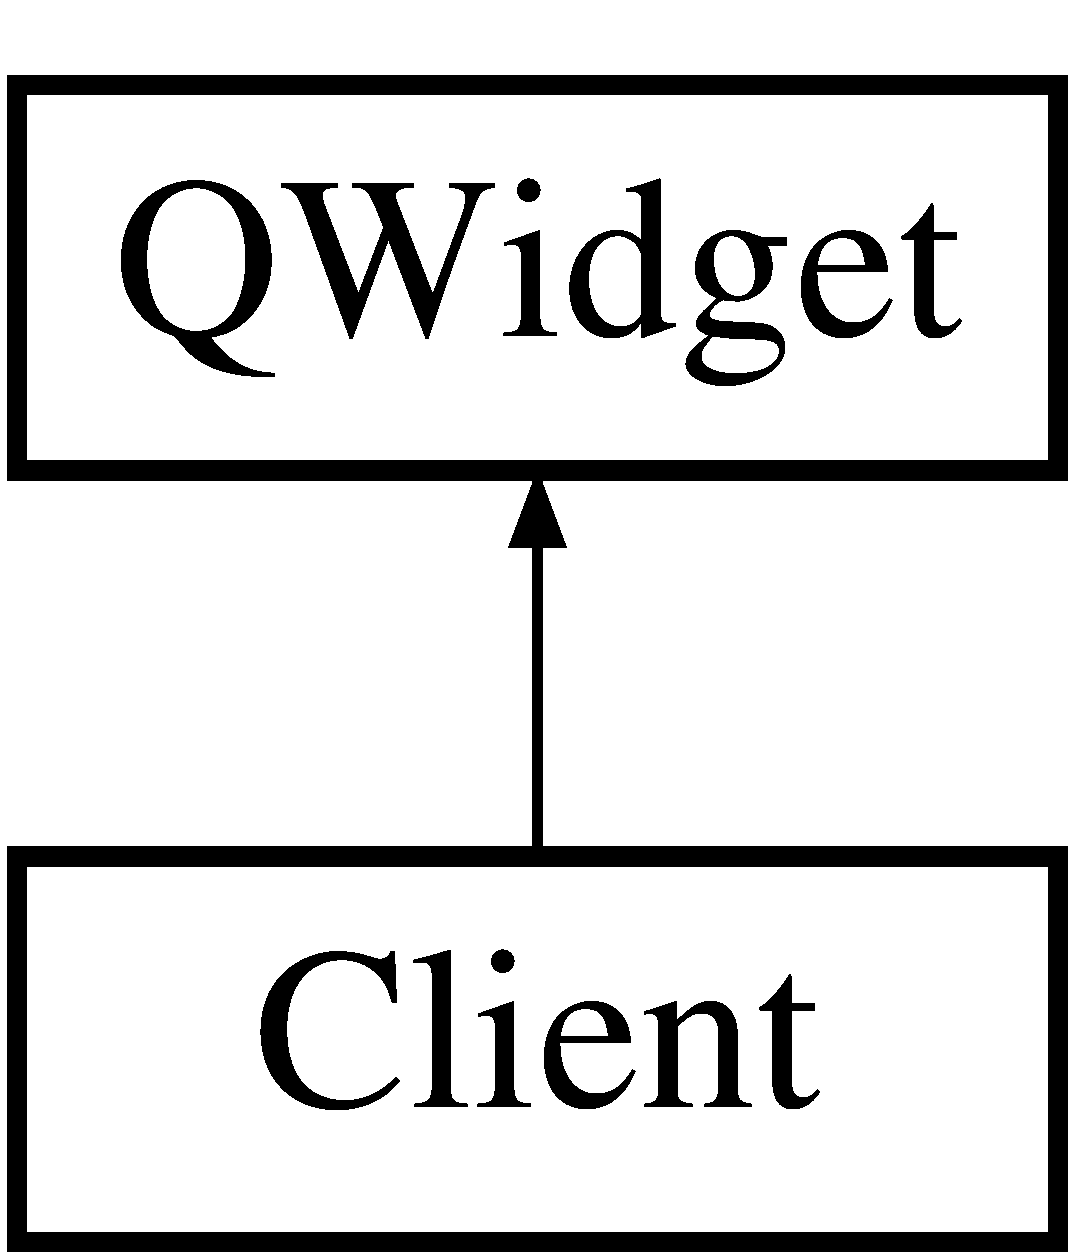
\includegraphics[height=2.000000cm]{class_client}
\end{center}
\end{figure}
\subsection*{Öffentliche Slots}
\begin{DoxyCompactItemize}
\item 
\hypertarget{class_client_a5f96334ebe2c8a22f6448cff80d027a5}{}\label{class_client_a5f96334ebe2c8a22f6448cff80d027a5} 
void \hyperlink{class_client_a5f96334ebe2c8a22f6448cff80d027a5}{on\+Exit\+Button\+Clicked} ()
\begin{DoxyCompactList}\small\item\em Beim Klicken des Schliessen-\/\+Button aufgerufene Handler-\/\+Methode. \end{DoxyCompactList}\item 
\hypertarget{class_client_aa56b217ce77d6e41f76474ed92378798}{}\label{class_client_aa56b217ce77d6e41f76474ed92378798} 
void \hyperlink{class_client_aa56b217ce77d6e41f76474ed92378798}{on\+Start\+Button\+Clicked} ()
\begin{DoxyCompactList}\small\item\em Beim Klicken des Starten-\/\+Button aufgerufene Handler-\/\+Methode. \end{DoxyCompactList}\item 
\hypertarget{class_client_a548c8d8b2eb95c3ecbec190495940b99}{}\label{class_client_a548c8d8b2eb95c3ecbec190495940b99} 
void \hyperlink{class_client_a548c8d8b2eb95c3ecbec190495940b99}{on\+Keyboard\+Clicked} ()
\begin{DoxyCompactList}\small\item\em Beim Klicken des Keyboard-\/\+Button aufgerufene Handler-\/\+Methode. \end{DoxyCompactList}\item 
\hypertarget{class_client_a8dbb1b513ea96c6016e97cb03d4e6b0d}{}\label{class_client_a8dbb1b513ea96c6016e97cb03d4e6b0d} 
void \hyperlink{class_client_a8dbb1b513ea96c6016e97cb03d4e6b0d}{on\+Runtime\+Changed} (int)
\begin{DoxyCompactList}\small\item\em Beim Bewegen oder Anklicken des Slider \char`\"{}\+Laufzeit\char`\"{} aufgerufene Handler-\/\+Methode. \end{DoxyCompactList}\item 
\hypertarget{class_client_afe033bbce94884369c9b488485f879ad}{}\label{class_client_afe033bbce94884369c9b488485f879ad} 
void \hyperlink{class_client_afe033bbce94884369c9b488485f879ad}{on\+Bandwidth\+Changed} (int)
\begin{DoxyCompactList}\small\item\em Beim Bewegen oder Anklicken des Slider \char`\"{}\+Bandbreite\char`\"{} aufgerufene Handler-\/\+Methode. \end{DoxyCompactList}\item 
\hypertarget{class_client_a01f6d4ddcb338116dc4a4ba320f47456}{}\label{class_client_a01f6d4ddcb338116dc4a4ba320f47456} 
void \hyperlink{class_client_a01f6d4ddcb338116dc4a4ba320f47456}{on\+Client\+Has\+Finished} ()
\begin{DoxyCompactList}\small\item\em Wird aufgerufen sobald der \hyperlink{class_client}{Client} keine Pakete mehr sendet, also beendet ist. \end{DoxyCompactList}\item 
void \hyperlink{class_client_a9699e2db43beff88b4694208c54c1b7f}{set\+IP} (Q\+String s)
\begin{DoxyCompactList}\small\item\em Setzt die I\+P-\/\+Adresse. \end{DoxyCompactList}\item 
Q\+String \hyperlink{class_client_a91bf1f59731649499365d8b18e6aee62}{get\+IP} ()
\begin{DoxyCompactList}\small\item\em Gibt die I\+P-\/\+Adresse zurück. \end{DoxyCompactList}\end{DoxyCompactItemize}
\subsection*{Öffentliche Methoden}
\begin{DoxyCompactItemize}
\item 
\hyperlink{class_client_ab9cb979d7fb7dd0bd3bf645279a6ffb5}{Client} (Q\+Widget $\ast$parent=0)
\begin{DoxyCompactList}\small\item\em \hyperlink{class_client}{Client} Konstruktor. \end{DoxyCompactList}\end{DoxyCompactItemize}


\subsection{Ausführliche Beschreibung}
Die Client-\/\+Klasse. 

\subsection{Beschreibung der Konstruktoren und Destruktoren}
\hypertarget{class_client_ab9cb979d7fb7dd0bd3bf645279a6ffb5}{}\label{class_client_ab9cb979d7fb7dd0bd3bf645279a6ffb5} 
\index{Client@{Client}!Client@{Client}}
\index{Client@{Client}!Client@{Client}}
\subsubsection{\texorpdfstring{Client()}{Client()}}
{\footnotesize\ttfamily Client\+::\+Client (\begin{DoxyParamCaption}\item[{Q\+Widget $\ast$}]{parent = {\ttfamily 0} }\end{DoxyParamCaption})\hspace{0.3cm}{\ttfamily [explicit]}}



\hyperlink{class_client}{Client} Konstruktor. 


\begin{DoxyParams}{Parameter}
{\em parent} & \\
\hline
\end{DoxyParams}


\subsection{Dokumentation der Elementfunktionen}
\hypertarget{class_client_a91bf1f59731649499365d8b18e6aee62}{}\label{class_client_a91bf1f59731649499365d8b18e6aee62} 
\index{Client@{Client}!get\+IP@{get\+IP}}
\index{get\+IP@{get\+IP}!Client@{Client}}
\subsubsection{\texorpdfstring{get\+IP}{getIP}}
{\footnotesize\ttfamily Q\+String Client\+::get\+IP (\begin{DoxyParamCaption}{ }\end{DoxyParamCaption})\hspace{0.3cm}{\ttfamily [slot]}}



Gibt die I\+P-\/\+Adresse zurück. 

\begin{DoxyReturn}{Rückgabe}
Die I\+P-\/\+Adresse als String im Format 192.\+168.\+0.\+40 
\end{DoxyReturn}
\hypertarget{class_client_a9699e2db43beff88b4694208c54c1b7f}{}\label{class_client_a9699e2db43beff88b4694208c54c1b7f} 
\index{Client@{Client}!set\+IP@{set\+IP}}
\index{set\+IP@{set\+IP}!Client@{Client}}
\subsubsection{\texorpdfstring{set\+IP}{setIP}}
{\footnotesize\ttfamily void Client\+::set\+IP (\begin{DoxyParamCaption}\item[{Q\+String}]{s }\end{DoxyParamCaption})\hspace{0.3cm}{\ttfamily [slot]}}



Setzt die I\+P-\/\+Adresse. 


\begin{DoxyParams}{Parameter}
{\em s} & Die I\+P-\/\+Adresse als String im Format 192.\+168.\+0.\+40 \\
\hline
\end{DoxyParams}


Die Dokumentation für diese Klasse wurde erzeugt aufgrund der Dateien\+:\begin{DoxyCompactItemize}
\item 
src/\hyperlink{client_8h}{client.\+h}\item 
src/client.\+cpp\end{DoxyCompactItemize}

\hypertarget{class_iperf_interface}{}\section{Iperf\+Interface Klassenreferenz}
\label{class_iperf_interface}\index{Iperf\+Interface@{Iperf\+Interface}}


Die Iperf\+Interface-\/\+Klasse.  




{\ttfamily \#include $<$iperfinterface.\+h$>$}

Klassendiagramm für Iperf\+Interface\+:\begin{figure}[H]
\begin{center}
\leavevmode
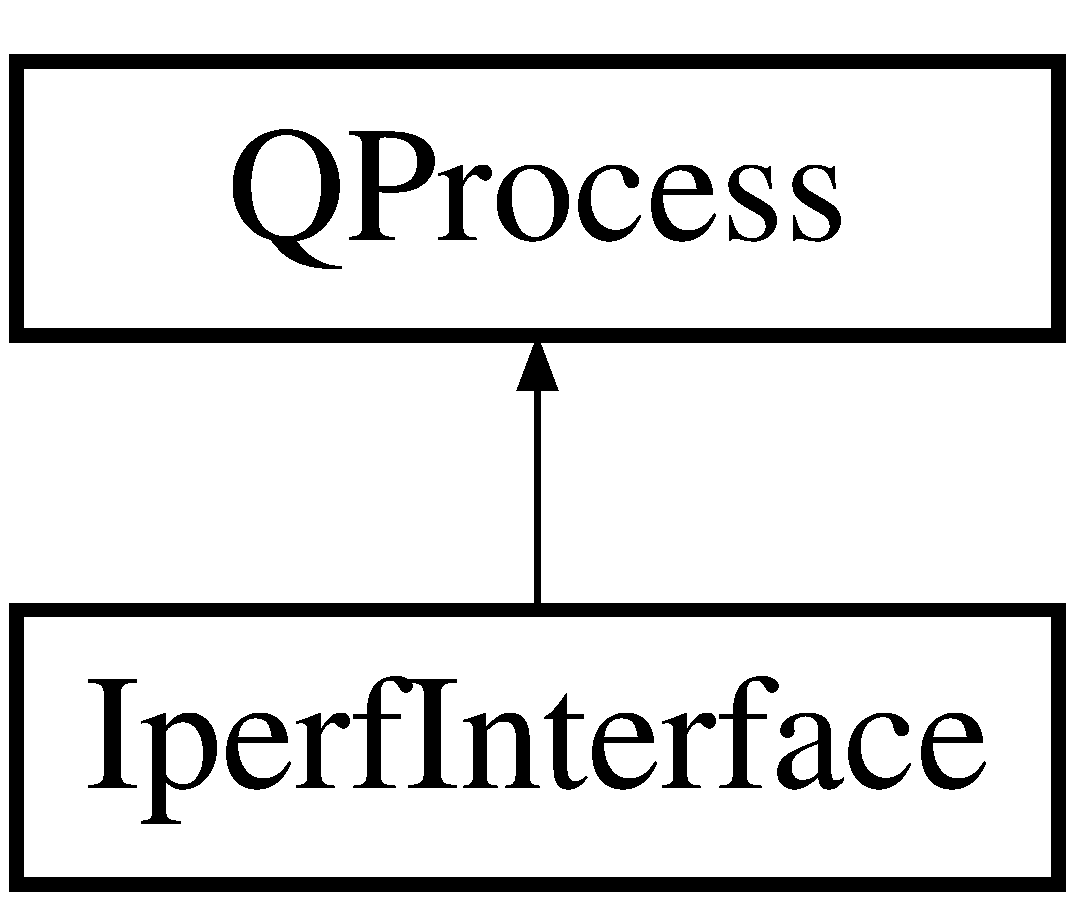
\includegraphics[height=2.000000cm]{class_iperf_interface}
\end{center}
\end{figure}
\subsection*{Öffentliche Slots}
\begin{DoxyCompactItemize}
\item 
\hypertarget{class_iperf_interface_a28845faae84e19418b0c2006785d93a7}{}\label{class_iperf_interface_a28845faae84e19418b0c2006785d93a7} 
void \hyperlink{class_iperf_interface_a28845faae84e19418b0c2006785d93a7}{process\+Ready\+Read\+Standard\+Output} ()
\begin{DoxyCompactList}\small\item\em Bei der Bereitschaft des Prozesses aufgerufene Handler-\/\+Methode. \end{DoxyCompactList}\item 
\hypertarget{class_iperf_interface_a9d82924212dac8a3cdd5ac074a99ec88}{}\label{class_iperf_interface_a9d82924212dac8a3cdd5ac074a99ec88} 
void \hyperlink{class_iperf_interface_a9d82924212dac8a3cdd5ac074a99ec88}{process\+File\+Changed} (const Q\+String \&)
\begin{DoxyCompactList}\small\item\em Beim Ändern der Logdatei aufgerufene Handler-\/\+Methode. \end{DoxyCompactList}\end{DoxyCompactItemize}
\subsection*{Signale}
\begin{DoxyCompactItemize}
\item 
\hypertarget{class_iperf_interface_a8a0e602fe96d401f2ce61cf71f99d8da}{}\label{class_iperf_interface_a8a0e602fe96d401f2ce61cf71f99d8da} 
void \hyperlink{class_iperf_interface_a8a0e602fe96d401f2ce61cf71f99d8da}{log\+Output} (const Q\+String \&)
\begin{DoxyCompactList}\small\item\em Signal wenn der Output geloggt wird. \end{DoxyCompactList}\item 
\hypertarget{class_iperf_interface_a7263bbb7d6ee2285331b030d36efe6c6}{}\label{class_iperf_interface_a7263bbb7d6ee2285331b030d36efe6c6} 
void \hyperlink{class_iperf_interface_a7263bbb7d6ee2285331b030d36efe6c6}{server\+Started\+Listening} ()
\begin{DoxyCompactList}\small\item\em Signal wenn Start des Servers abgeschlossen ist. \end{DoxyCompactList}\item 
\hypertarget{class_iperf_interface_a51b38e37b0b7d1feb8ba02e34d7a2336}{}\label{class_iperf_interface_a51b38e37b0b7d1feb8ba02e34d7a2336} 
void \hyperlink{class_iperf_interface_a51b38e37b0b7d1feb8ba02e34d7a2336}{connection\+Established} ()
\begin{DoxyCompactList}\small\item\em Signal wenn die Verbindung zwischen \hyperlink{class_client}{Client} und \hyperlink{class_server}{Server} aufgebaut ist. \end{DoxyCompactList}\item 
\hypertarget{class_iperf_interface_a58a0afd22191a9e63d6fd8e8a047ce5b}{}\label{class_iperf_interface_a58a0afd22191a9e63d6fd8e8a047ce5b} 
void \hyperlink{class_iperf_interface_a58a0afd22191a9e63d6fd8e8a047ce5b}{connection\+Closed} ()
\begin{DoxyCompactList}\small\item\em Signal wenn die Verbindung zwischen \hyperlink{class_client}{Client} und \hyperlink{class_server}{Server} geschlossen wurde. \end{DoxyCompactList}\end{DoxyCompactItemize}
\subsection*{Öffentliche Methoden}
\begin{DoxyCompactItemize}
\item 
\hyperlink{class_iperf_interface_a29d7d64376a399ce741da79c1a9c544c}{Iperf\+Interface} (Q\+String initial\+Arguments=Q\+String(), Q\+String log\+Path\+And\+Filename=Q\+String(\char`\"{}/tmp/iperf3.\+log\char`\"{}))
\begin{DoxyCompactList}\small\item\em Der Iperf\+Interface-\/\+Konstruktor. \end{DoxyCompactList}\item 
void \hyperlink{class_iperf_interface_a4aa4821c81d91e93afe3f5ae2c24bacf}{set\+Initial\+Arguments} (Q\+String initial\+Arguments)
\begin{DoxyCompactList}\small\item\em Setzt die Argumente-\/\+Liste. \end{DoxyCompactList}\item 
Q\+String \hyperlink{class_iperf_interface_a93b05412f77de1fc4cb57e5b03f378dd}{get\+Initial\+Arguments} ()
\begin{DoxyCompactList}\small\item\em Gibt die Argumente-\/\+Liste als String zurück. \end{DoxyCompactList}\item 
Q\+String \hyperlink{class_iperf_interface_a62e1dad7ad79df8307384b76a14f6eed}{get\+Log\+Path\+And\+Filename} ()
\begin{DoxyCompactList}\small\item\em Gibt den Pfad zur Logdatei zurück. \end{DoxyCompactList}\item 
void \hyperlink{class_iperf_interface_a012e33d4dcb33373c302cf1282b3056b}{set\+Server\+Is\+Listening} (bool server\+Is\+Listening)
\begin{DoxyCompactList}\small\item\em Setzt den \hyperlink{class_server}{Server} auf \char`\"{}\+Listening\char`\"{}. \end{DoxyCompactList}\item 
bool \hyperlink{class_iperf_interface_a68b6291bcbf2ad413f4efa00ebf9b66d}{get\+Is\+Server\+Listening} ()
\begin{DoxyCompactList}\small\item\em Gibt zurück ob der \hyperlink{class_server}{Server} auf \char`\"{}\+Listening\char`\"{} gesetzt ist. \end{DoxyCompactList}\item 
Q\+Map$<$ Q\+String, Q\+String $>$ \hyperlink{class_iperf_interface_a81faf533ca54a96e9fa33006d50830bd}{get\+Network\+Interfaces} ()
\begin{DoxyCompactList}\small\item\em Gibt die Netzwerkschnittstellen als Map zurück. \end{DoxyCompactList}\item 
\hypertarget{class_iperf_interface_a0f982e150bc78c9d7413be362a9c5bfe}{}\label{class_iperf_interface_a0f982e150bc78c9d7413be362a9c5bfe} 
void \hyperlink{class_iperf_interface_a0f982e150bc78c9d7413be362a9c5bfe}{run} ()
\begin{DoxyCompactList}\small\item\em Startet das Kommandozeilenprogramm iperf3. \end{DoxyCompactList}\end{DoxyCompactItemize}


\subsection{Ausführliche Beschreibung}
Die Iperf\+Interface-\/\+Klasse. 

\subsection{Beschreibung der Konstruktoren und Destruktoren}
\hypertarget{class_iperf_interface_a29d7d64376a399ce741da79c1a9c544c}{}\label{class_iperf_interface_a29d7d64376a399ce741da79c1a9c544c} 
\index{Iperf\+Interface@{Iperf\+Interface}!Iperf\+Interface@{Iperf\+Interface}}
\index{Iperf\+Interface@{Iperf\+Interface}!Iperf\+Interface@{Iperf\+Interface}}
\subsubsection{\texorpdfstring{Iperf\+Interface()}{IperfInterface()}}
{\footnotesize\ttfamily Iperf\+Interface\+::\+Iperf\+Interface (\begin{DoxyParamCaption}\item[{Q\+String}]{initial\+Arguments = {\ttfamily QString()},  }\item[{Q\+String}]{log\+Path\+And\+Filename = {\ttfamily QString(\char`\"{}/tmp/iperf3.log\char`\"{})} }\end{DoxyParamCaption})}



Der Iperf\+Interface-\/\+Konstruktor. 


\begin{DoxyParams}{Parameter}
{\em initial\+Arguments} & Die Argumente-\/\+Liste, welche an das Kommandozeilenprogramm übermittelt werden. \\
\hline
{\em log\+Path\+And\+Filename} & Der Pfad zur Logdatei. \\
\hline
\end{DoxyParams}


\subsection{Dokumentation der Elementfunktionen}
\hypertarget{class_iperf_interface_a93b05412f77de1fc4cb57e5b03f378dd}{}\label{class_iperf_interface_a93b05412f77de1fc4cb57e5b03f378dd} 
\index{Iperf\+Interface@{Iperf\+Interface}!get\+Initial\+Arguments@{get\+Initial\+Arguments}}
\index{get\+Initial\+Arguments@{get\+Initial\+Arguments}!Iperf\+Interface@{Iperf\+Interface}}
\subsubsection{\texorpdfstring{get\+Initial\+Arguments()}{getInitialArguments()}}
{\footnotesize\ttfamily Q\+String Iperf\+Interface\+::get\+Initial\+Arguments (\begin{DoxyParamCaption}{ }\end{DoxyParamCaption})}



Gibt die Argumente-\/\+Liste als String zurück. 

\begin{DoxyReturn}{Rückgabe}
Die Argumente-\/\+Liste als String. 
\end{DoxyReturn}
\hypertarget{class_iperf_interface_a68b6291bcbf2ad413f4efa00ebf9b66d}{}\label{class_iperf_interface_a68b6291bcbf2ad413f4efa00ebf9b66d} 
\index{Iperf\+Interface@{Iperf\+Interface}!get\+Is\+Server\+Listening@{get\+Is\+Server\+Listening}}
\index{get\+Is\+Server\+Listening@{get\+Is\+Server\+Listening}!Iperf\+Interface@{Iperf\+Interface}}
\subsubsection{\texorpdfstring{get\+Is\+Server\+Listening()}{getIsServerListening()}}
{\footnotesize\ttfamily bool Iperf\+Interface\+::get\+Is\+Server\+Listening (\begin{DoxyParamCaption}{ }\end{DoxyParamCaption})}



Gibt zurück ob der \hyperlink{class_server}{Server} auf \char`\"{}\+Listening\char`\"{} gesetzt ist. 

\begin{DoxyReturn}{Rückgabe}
Den Status \char`\"{}\+Listening\char`\"{} 
\end{DoxyReturn}
\hypertarget{class_iperf_interface_a62e1dad7ad79df8307384b76a14f6eed}{}\label{class_iperf_interface_a62e1dad7ad79df8307384b76a14f6eed} 
\index{Iperf\+Interface@{Iperf\+Interface}!get\+Log\+Path\+And\+Filename@{get\+Log\+Path\+And\+Filename}}
\index{get\+Log\+Path\+And\+Filename@{get\+Log\+Path\+And\+Filename}!Iperf\+Interface@{Iperf\+Interface}}
\subsubsection{\texorpdfstring{get\+Log\+Path\+And\+Filename()}{getLogPathAndFilename()}}
{\footnotesize\ttfamily Q\+String Iperf\+Interface\+::get\+Log\+Path\+And\+Filename (\begin{DoxyParamCaption}{ }\end{DoxyParamCaption})}



Gibt den Pfad zur Logdatei zurück. 

\begin{DoxyReturn}{Rückgabe}
Der Pfad als String. 
\end{DoxyReturn}
\hypertarget{class_iperf_interface_a81faf533ca54a96e9fa33006d50830bd}{}\label{class_iperf_interface_a81faf533ca54a96e9fa33006d50830bd} 
\index{Iperf\+Interface@{Iperf\+Interface}!get\+Network\+Interfaces@{get\+Network\+Interfaces}}
\index{get\+Network\+Interfaces@{get\+Network\+Interfaces}!Iperf\+Interface@{Iperf\+Interface}}
\subsubsection{\texorpdfstring{get\+Network\+Interfaces()}{getNetworkInterfaces()}}
{\footnotesize\ttfamily Q\+Map$<$ Q\+String, Q\+String $>$ Iperf\+Interface\+::get\+Network\+Interfaces (\begin{DoxyParamCaption}{ }\end{DoxyParamCaption})}



Gibt die Netzwerkschnittstellen als Map zurück. 

\begin{DoxyReturn}{Rückgabe}
Die Netzwerkschnittstellen 
\end{DoxyReturn}
\hypertarget{class_iperf_interface_a4aa4821c81d91e93afe3f5ae2c24bacf}{}\label{class_iperf_interface_a4aa4821c81d91e93afe3f5ae2c24bacf} 
\index{Iperf\+Interface@{Iperf\+Interface}!set\+Initial\+Arguments@{set\+Initial\+Arguments}}
\index{set\+Initial\+Arguments@{set\+Initial\+Arguments}!Iperf\+Interface@{Iperf\+Interface}}
\subsubsection{\texorpdfstring{set\+Initial\+Arguments()}{setInitialArguments()}}
{\footnotesize\ttfamily void Iperf\+Interface\+::set\+Initial\+Arguments (\begin{DoxyParamCaption}\item[{Q\+String}]{initial\+Arguments }\end{DoxyParamCaption})}



Setzt die Argumente-\/\+Liste. 


\begin{DoxyParams}{Parameter}
{\em initial\+Arguments} & Die Argumente-\/\+Liste als String. \\
\hline
\end{DoxyParams}
\hypertarget{class_iperf_interface_a012e33d4dcb33373c302cf1282b3056b}{}\label{class_iperf_interface_a012e33d4dcb33373c302cf1282b3056b} 
\index{Iperf\+Interface@{Iperf\+Interface}!set\+Server\+Is\+Listening@{set\+Server\+Is\+Listening}}
\index{set\+Server\+Is\+Listening@{set\+Server\+Is\+Listening}!Iperf\+Interface@{Iperf\+Interface}}
\subsubsection{\texorpdfstring{set\+Server\+Is\+Listening()}{setServerIsListening()}}
{\footnotesize\ttfamily void Iperf\+Interface\+::set\+Server\+Is\+Listening (\begin{DoxyParamCaption}\item[{bool}]{server\+Is\+Listening }\end{DoxyParamCaption})}



Setzt den \hyperlink{class_server}{Server} auf \char`\"{}\+Listening\char`\"{}. 


\begin{DoxyParams}{Parameter}
{\em server\+Is\+Listening} & \\
\hline
\end{DoxyParams}


Die Dokumentation für diese Klasse wurde erzeugt aufgrund der Dateien\+:\begin{DoxyCompactItemize}
\item 
src/\hyperlink{iperfinterface_8h}{iperfinterface.\+h}\item 
src/iperfinterface.\+cpp\end{DoxyCompactItemize}

\hypertarget{class_num_pad}{}\section{Num\+Pad Class Reference}
\label{class_num_pad}\index{Num\+Pad@{Num\+Pad}}
Inheritance diagram for Num\+Pad\+:\begin{figure}[H]
\begin{center}
\leavevmode
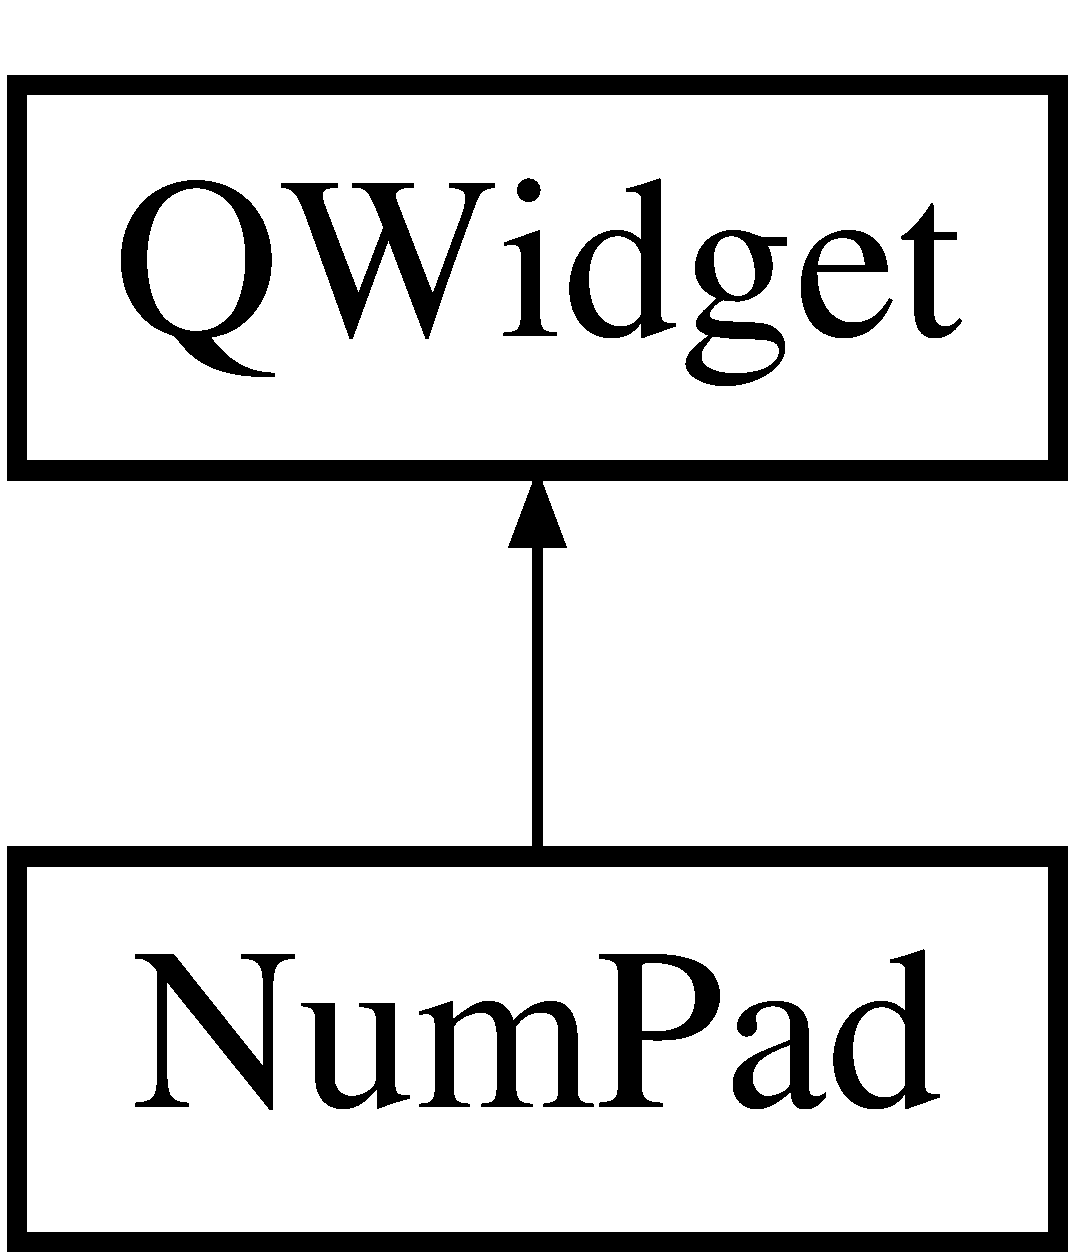
\includegraphics[height=2.000000cm]{class_num_pad}
\end{center}
\end{figure}
\subsection*{Public Slots}
\begin{DoxyCompactItemize}
\item 
\hypertarget{class_num_pad_ac6620373f360b666b71108b13946013a}{}\label{class_num_pad_ac6620373f360b666b71108b13946013a} 
void {\bfseries on\+Button\+Zero\+Clicked} ()
\item 
\hypertarget{class_num_pad_a6623d11d0e41f47e476f5e99a0d4eb71}{}\label{class_num_pad_a6623d11d0e41f47e476f5e99a0d4eb71} 
void {\bfseries on\+Button\+One\+Clicked} ()
\item 
\hypertarget{class_num_pad_a16eb90e6203c9d59eb0c6ea2697100c2}{}\label{class_num_pad_a16eb90e6203c9d59eb0c6ea2697100c2} 
void {\bfseries on\+Button\+Two\+Clicked} ()
\item 
\hypertarget{class_num_pad_a7e4ddab2ee993b84198b589b16305a76}{}\label{class_num_pad_a7e4ddab2ee993b84198b589b16305a76} 
void {\bfseries on\+Button\+Three\+Clicked} ()
\item 
\hypertarget{class_num_pad_afd185aa4de995f81384ca9d6c0f52af5}{}\label{class_num_pad_afd185aa4de995f81384ca9d6c0f52af5} 
void {\bfseries on\+Button\+Four\+Clicked} ()
\item 
\hypertarget{class_num_pad_aa494f765620859681fa7daac1b6dbc57}{}\label{class_num_pad_aa494f765620859681fa7daac1b6dbc57} 
void {\bfseries on\+Button\+Five\+Clicked} ()
\item 
\hypertarget{class_num_pad_a0eec28eb14ac08a0bd90eebcd43bfea6}{}\label{class_num_pad_a0eec28eb14ac08a0bd90eebcd43bfea6} 
void {\bfseries on\+Button\+Six\+Clicked} ()
\item 
\hypertarget{class_num_pad_a249c3837cc94eea7e2fdec57d78e1d6b}{}\label{class_num_pad_a249c3837cc94eea7e2fdec57d78e1d6b} 
void {\bfseries on\+Button\+Seven\+Clicked} ()
\item 
\hypertarget{class_num_pad_aefad78a1724a0962dc66df3f8b434a8a}{}\label{class_num_pad_aefad78a1724a0962dc66df3f8b434a8a} 
void {\bfseries on\+Button\+Eight\+Clicked} ()
\item 
\hypertarget{class_num_pad_a453339b8ce818824204f96607708c916}{}\label{class_num_pad_a453339b8ce818824204f96607708c916} 
void {\bfseries on\+Button\+Nine\+Clicked} ()
\item 
\hypertarget{class_num_pad_a153332f9a9b050037329d054d8cac6ae}{}\label{class_num_pad_a153332f9a9b050037329d054d8cac6ae} 
void {\bfseries on\+Button\+Dot\+Clicked} ()
\item 
\hypertarget{class_num_pad_abc4841a30a7777e207aebeb6020d9194}{}\label{class_num_pad_abc4841a30a7777e207aebeb6020d9194} 
void {\bfseries on\+Button\+Done\+Clicked} ()
\item 
\hypertarget{class_num_pad_a8e5af4566f4c3e5574a6867877ee795b}{}\label{class_num_pad_a8e5af4566f4c3e5574a6867877ee795b} 
void {\bfseries on\+Button\+Bksp\+Clicked} ()
\end{DoxyCompactItemize}
\subsection*{Public Member Functions}
\begin{DoxyCompactItemize}
\item 
\hypertarget{class_num_pad_ac35bfd6bb99a182c9073d80a09f3baf9}{}\label{class_num_pad_ac35bfd6bb99a182c9073d80a09f3baf9} 
{\bfseries Num\+Pad} (\hyperlink{class_client}{Client} $\ast$c)
\end{DoxyCompactItemize}
\subsection*{Public Attributes}
\begin{DoxyCompactItemize}
\item 
\hypertarget{class_num_pad_aeba02dbc3ca834bbd75f817855f5ecfb}{}\label{class_num_pad_aeba02dbc3ca834bbd75f817855f5ecfb} 
\hyperlink{class_client}{Client} $\ast$ {\bfseries client}
\end{DoxyCompactItemize}


The documentation for this class was generated from the following files\+:\begin{DoxyCompactItemize}
\item 
src/numpad.\+h\item 
src/numpad.\+cpp\end{DoxyCompactItemize}

\hypertarget{class_server}{}\section{Server Class Reference}
\label{class_server}\index{Server@{Server}}
Inheritance diagram for Server\+:\begin{figure}[H]
\begin{center}
\leavevmode
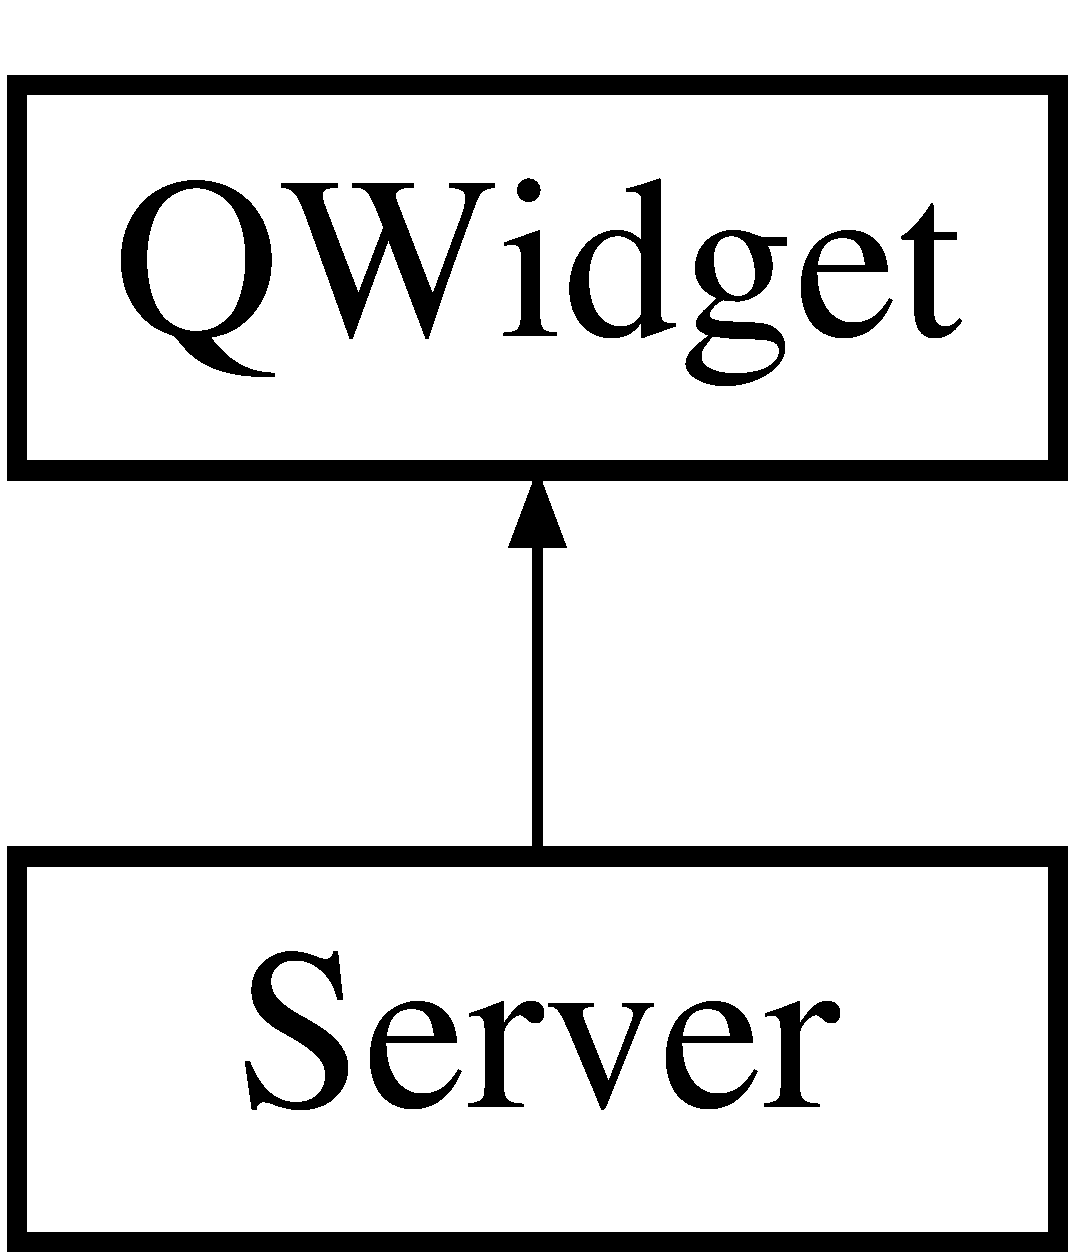
\includegraphics[height=2.000000cm]{class_server}
\end{center}
\end{figure}
\subsection*{Public Slots}
\begin{DoxyCompactItemize}
\item 
\hypertarget{class_server_a99f9b2f3521fb22772a61baf4f3c7bdc}{}\label{class_server_a99f9b2f3521fb22772a61baf4f3c7bdc} 
void {\bfseries on\+Exit\+Button\+Clicked} ()
\item 
\hypertarget{class_server_abe8ac23afc4d282f89ec9fac8e7bf7f3}{}\label{class_server_abe8ac23afc4d282f89ec9fac8e7bf7f3} 
void {\bfseries on\+Start\+Button\+Clicked} ()
\end{DoxyCompactItemize}
\subsection*{Public Member Functions}
\begin{DoxyCompactItemize}
\item 
\hypertarget{class_server_a0bf03b27b29ae4b969ec903f95041a17}{}\label{class_server_a0bf03b27b29ae4b969ec903f95041a17} 
{\bfseries Server} (Q\+Widget $\ast$parent=0)
\end{DoxyCompactItemize}


The documentation for this class was generated from the following files\+:\begin{DoxyCompactItemize}
\item 
src/server.\+h\item 
src/server.\+cpp\end{DoxyCompactItemize}

\hypertarget{class_traffic_light}{}\section{Traffic\+Light Klassenreferenz}
\label{class_traffic_light}\index{Traffic\+Light@{Traffic\+Light}}


Die Traffic\+Light-\/\+Klasse.  




{\ttfamily \#include $<$trafficlight.\+h$>$}

Klassendiagramm für Traffic\+Light\+:\begin{figure}[H]
\begin{center}
\leavevmode
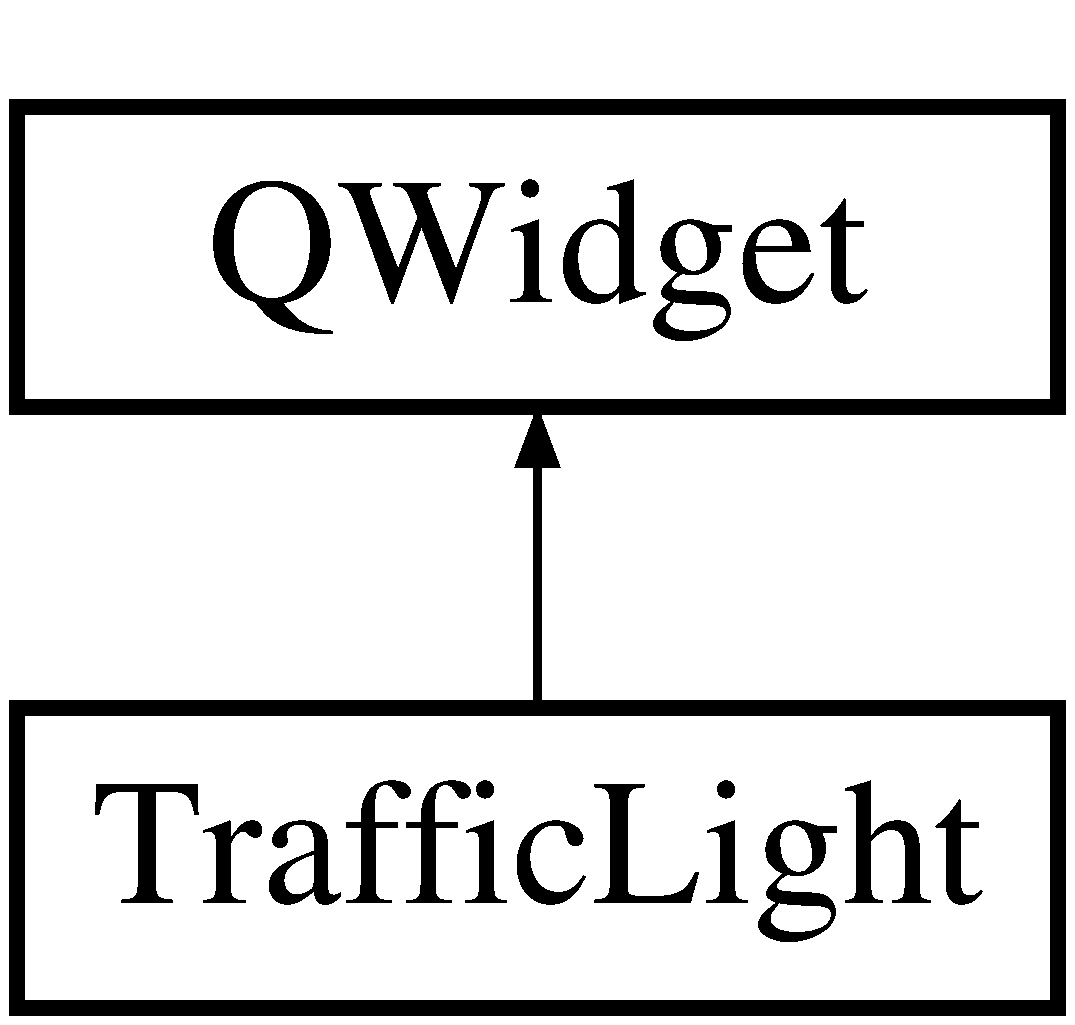
\includegraphics[height=2.000000cm]{class_traffic_light}
\end{center}
\end{figure}
\subsection*{Öffentliche Typen}
\begin{DoxyCompactItemize}
\item 
\hypertarget{class_traffic_light_a52ce5d9c3d0ec5aad2884db90fc10876}{}\label{class_traffic_light_a52ce5d9c3d0ec5aad2884db90fc10876} 
enum \hyperlink{class_traffic_light_a52ce5d9c3d0ec5aad2884db90fc10876}{color} \{ {\bfseries green}, 
{\bfseries red}, 
{\bfseries yellow}
 \}\begin{DoxyCompactList}\small\item\em Die drei Farben Grün, Rot, Gelb. \end{DoxyCompactList}
\end{DoxyCompactItemize}
\subsection*{Öffentliche Methoden}
\begin{DoxyCompactItemize}
\item 
\hyperlink{class_traffic_light_aa018a0285c92c087e48d3b16be3088ca}{Traffic\+Light} (Q\+Widget $\ast$parent=0)
\begin{DoxyCompactList}\small\item\em Der Traffic\+Light-\/\+Konstruktor. \end{DoxyCompactList}\item 
void \hyperlink{class_traffic_light_ad1e030e87446be2c976f5aedb4f511d5}{set\+Color} (\hyperlink{class_traffic_light_a52ce5d9c3d0ec5aad2884db90fc10876}{color} c)
\begin{DoxyCompactList}\small\item\em Setzt die Farbe. \end{DoxyCompactList}\end{DoxyCompactItemize}


\subsection{Ausführliche Beschreibung}
Die Traffic\+Light-\/\+Klasse. 

\subsection{Beschreibung der Konstruktoren und Destruktoren}
\hypertarget{class_traffic_light_aa018a0285c92c087e48d3b16be3088ca}{}\label{class_traffic_light_aa018a0285c92c087e48d3b16be3088ca} 
\index{Traffic\+Light@{Traffic\+Light}!Traffic\+Light@{Traffic\+Light}}
\index{Traffic\+Light@{Traffic\+Light}!Traffic\+Light@{Traffic\+Light}}
\subsubsection{\texorpdfstring{Traffic\+Light()}{TrafficLight()}}
{\footnotesize\ttfamily Traffic\+Light\+::\+Traffic\+Light (\begin{DoxyParamCaption}\item[{Q\+Widget $\ast$}]{parent = {\ttfamily 0} }\end{DoxyParamCaption})\hspace{0.3cm}{\ttfamily [explicit]}}



Der Traffic\+Light-\/\+Konstruktor. 


\begin{DoxyParams}{Parameter}
{\em parent} & \\
\hline
\end{DoxyParams}


\subsection{Dokumentation der Elementfunktionen}
\hypertarget{class_traffic_light_ad1e030e87446be2c976f5aedb4f511d5}{}\label{class_traffic_light_ad1e030e87446be2c976f5aedb4f511d5} 
\index{Traffic\+Light@{Traffic\+Light}!set\+Color@{set\+Color}}
\index{set\+Color@{set\+Color}!Traffic\+Light@{Traffic\+Light}}
\subsubsection{\texorpdfstring{set\+Color()}{setColor()}}
{\footnotesize\ttfamily void Traffic\+Light\+::set\+Color (\begin{DoxyParamCaption}\item[{\hyperlink{class_traffic_light_a52ce5d9c3d0ec5aad2884db90fc10876}{Traffic\+Light\+::color}}]{c }\end{DoxyParamCaption})}



Setzt die Farbe. 


\begin{DoxyParams}{Parameter}
{\em c} & \\
\hline
\end{DoxyParams}


Die Dokumentation für diese Klasse wurde erzeugt aufgrund der Dateien\+:\begin{DoxyCompactItemize}
\item 
src/\hyperlink{trafficlight_8h}{trafficlight.\+h}\item 
src/trafficlight.\+cpp\end{DoxyCompactItemize}

\hypertarget{class_welcome_screen}{}\section{Welcome\+Screen Class Reference}
\label{class_welcome_screen}\index{Welcome\+Screen@{Welcome\+Screen}}
Inheritance diagram for Welcome\+Screen\+:\begin{figure}[H]
\begin{center}
\leavevmode
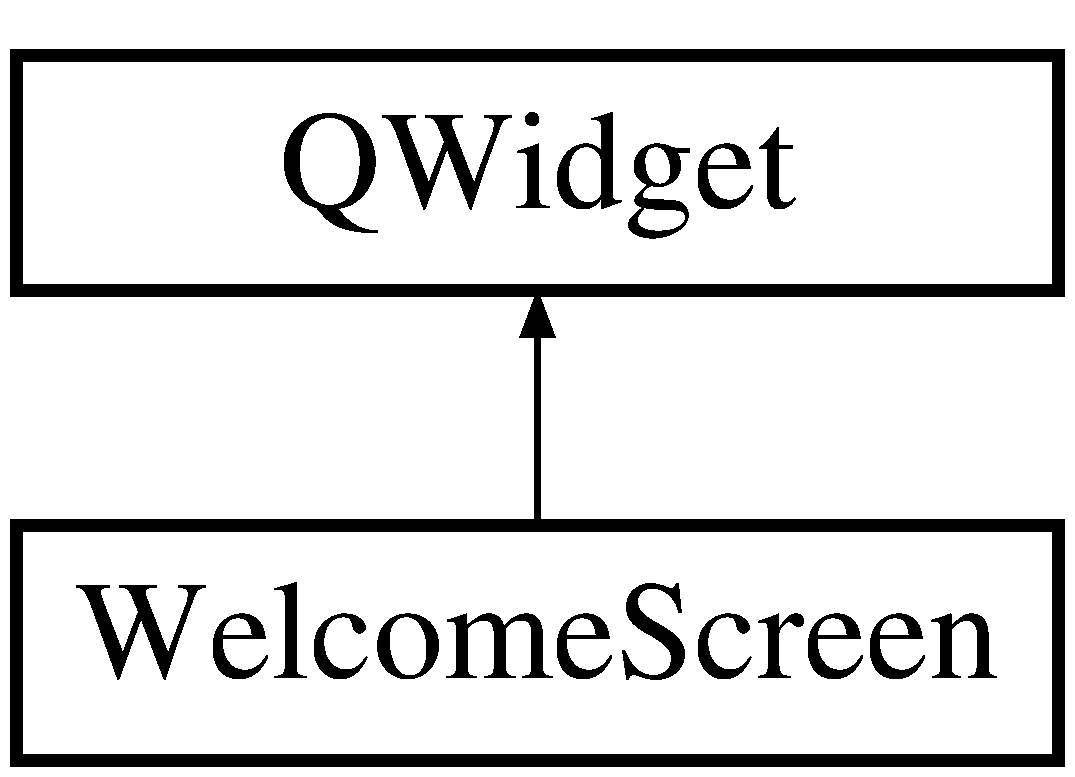
\includegraphics[height=2.000000cm]{class_welcome_screen}
\end{center}
\end{figure}
\subsection*{Public Slots}
\begin{DoxyCompactItemize}
\item 
\hypertarget{class_welcome_screen_adccaa9a1534c67f1fcd43245ff689b9e}{}\label{class_welcome_screen_adccaa9a1534c67f1fcd43245ff689b9e} 
void {\bfseries on\+Client\+Button\+Clicked} ()
\item 
\hypertarget{class_welcome_screen_ad4561643cb7feb6ad60e1daa097653d8}{}\label{class_welcome_screen_ad4561643cb7feb6ad60e1daa097653d8} 
void {\bfseries on\+Server\+Button\+Clicked} ()
\item 
\hypertarget{class_welcome_screen_a587ba35bfff39970d795906f253a52f8}{}\label{class_welcome_screen_a587ba35bfff39970d795906f253a52f8} 
void {\bfseries on\+Exit\+Button\+Clicked} ()
\end{DoxyCompactItemize}
\subsection*{Public Member Functions}
\begin{DoxyCompactItemize}
\item 
\hypertarget{class_welcome_screen_a5935d49d3bc2f3aae45db144bbbd4db2}{}\label{class_welcome_screen_a5935d49d3bc2f3aae45db144bbbd4db2} 
{\bfseries Welcome\+Screen} (Q\+Widget $\ast$parent=0)
\end{DoxyCompactItemize}


The documentation for this class was generated from the following files\+:\begin{DoxyCompactItemize}
\item 
src/welcomescreen.\+h\item 
src/welcomescreen.\+cpp\end{DoxyCompactItemize}

\chapter{Datei-\/\+Dokumentation}
\hypertarget{client_8h}{}\section{src/client.h File Reference}
\label{client_8h}\index{src/client.\+h@{src/client.\+h}}


A brief description about this header file.  


{\ttfamily \#include $<$Q\+Widget$>$}\newline
\subsection*{Classes}
\begin{DoxyCompactItemize}
\item 
class \hyperlink{class_client}{Client}
\begin{DoxyCompactList}\small\item\em The \hyperlink{class_client}{Client} class. \end{DoxyCompactList}\end{DoxyCompactItemize}


\subsection{Detailed Description}
A brief description about this header file. 

A long description about this header file.

\begin{DoxyAuthor}{Author}
Andreas Hueber 

Thomas Breuss 
\end{DoxyAuthor}

\hypertarget{iperfinterface_8h}{}\section{src/iperfinterface.h-\/\+Dateireferenz}
\label{iperfinterface_8h}\index{src/iperfinterface.\+h@{src/iperfinterface.\+h}}


Die Schnittstellen-\/\+Klasse für iperf3.  


{\ttfamily \#include $<$Q\+Byte\+Array$>$}\newline
{\ttfamily \#include $<$Q\+Debug$>$}\newline
{\ttfamily \#include $<$Q\+File$>$}\newline
{\ttfamily \#include $<$Q\+File\+System\+Watcher$>$}\newline
{\ttfamily \#include $<$Q\+Map$>$}\newline
{\ttfamily \#include $<$Q\+Object$>$}\newline
{\ttfamily \#include $<$Q\+Process$>$}\newline
{\ttfamily \#include $<$Q\+Reg\+Exp$>$}\newline
{\ttfamily \#include $<$Q\+String$>$}\newline
{\ttfamily \#include $<$Q\+String\+List$>$}\newline
{\ttfamily \#include $<$Q\+Text\+Stream$>$}\newline
{\ttfamily \#include $<$Qt\+Network$>$}\newline
\subsection*{Klassen}
\begin{DoxyCompactItemize}
\item 
class \hyperlink{class_iperf_interface}{Iperf\+Interface}
\begin{DoxyCompactList}\small\item\em Die Iperf\+Interface-\/\+Klasse. \end{DoxyCompactList}\end{DoxyCompactItemize}
\subsection*{Makrodefinitionen}
\begin{DoxyCompactItemize}
\item 
\hypertarget{iperfinterface_8h_ac2abe18781c7157acb0ad443d3bfefa6}{}\label{iperfinterface_8h_ac2abe18781c7157acb0ad443d3bfefa6} 
\#define {\bfseries I\+P\+E\+R\+F\+\_\+\+P\+A\+T\+H\+\_\+\+A\+N\+D\+\_\+\+F\+I\+L\+E\+N\+A\+ME}~\char`\"{}/usr/bin/iperf3\char`\"{}
\item 
\hypertarget{iperfinterface_8h_a2864939d4470c04aa2483de3fa15b984}{}\label{iperfinterface_8h_a2864939d4470c04aa2483de3fa15b984} 
\#define {\bfseries M\+S\+G\+\_\+\+S\+E\+R\+V\+E\+R\+\_\+\+L\+I\+S\+T\+E\+N\+I\+NG}~\char`\"{}Server listening on U\+DP port \mbox{[}0-\/9\mbox{]}+\char`\"{}
\item 
\hypertarget{iperfinterface_8h_a84ad75c7007d50b2b4fa18beabe5d58f}{}\label{iperfinterface_8h_a84ad75c7007d50b2b4fa18beabe5d58f} 
\#define {\bfseries M\+S\+G\+\_\+\+S\+E\+R\+V\+E\+R\+\_\+\+H\+A\+S\+\_\+\+T\+E\+R\+M\+I\+N\+A\+T\+ED}~\char`\"{}the server has terminated\char`\"{}
\item 
\hypertarget{iperfinterface_8h_a35c703c8e2f12c9742fbdf33de1d9f14}{}\label{iperfinterface_8h_a35c703c8e2f12c9742fbdf33de1d9f14} 
\#define {\bfseries M\+S\+G\+\_\+\+C\+O\+N\+N\+E\+C\+T\+I\+O\+N\+\_\+\+E\+S\+T\+A\+B\+L\+I\+S\+H\+ED}~\char`\"{}Accepted connection from\char`\"{}
\item 
\hypertarget{iperfinterface_8h_a255f9bf3ec5cfd78d02af36b4b849e09}{}\label{iperfinterface_8h_a255f9bf3ec5cfd78d02af36b4b849e09} 
\#define {\bfseries M\+S\+G\+\_\+\+C\+O\+N\+N\+E\+C\+T\+I\+O\+N\+\_\+\+C\+L\+O\+S\+ED}~\char`\"{}Lost/Total Datagrams\char`\"{}
\item 
\hypertarget{iperfinterface_8h_a66011f0797a15e752c39643919c885b6}{}\label{iperfinterface_8h_a66011f0797a15e752c39643919c885b6} 
\#define {\bfseries M\+S\+G\+\_\+\+S\+O\+C\+K\+E\+T\+\_\+\+U\+N\+E\+X\+P\+E\+C\+T\+E\+D\+L\+Y\+\_\+\+C\+L\+O\+S\+ED}~\char`\"{}control socket has closed unexpectedly\char`\"{}
\item 
\hypertarget{iperfinterface_8h_ad5aeb6d0cc27d1b17afeed94c684a040}{}\label{iperfinterface_8h_ad5aeb6d0cc27d1b17afeed94c684a040} 
\#define {\bfseries M\+S\+G\+\_\+\+C\+L\+I\+E\+N\+T\+\_\+\+C\+O\+N\+N\+E\+C\+T\+I\+O\+N\+\_\+\+R\+E\+F\+U\+S\+ED}~\char`\"{}Connection refused\char`\"{}
\item 
\hypertarget{iperfinterface_8h_af963d447dfb9fa35c3e2a82a49bb400c}{}\label{iperfinterface_8h_af963d447dfb9fa35c3e2a82a49bb400c} 
\#define {\bfseries M\+S\+G\+\_\+\+C\+L\+I\+E\+N\+T\+\_\+\+H\+A\+S\+\_\+\+T\+E\+R\+M\+I\+N\+A\+T\+ED}~\char`\"{}iperf3\+: the client has terminated\char`\"{}
\item 
\hypertarget{iperfinterface_8h_a704552ef03f196ac43b20baa26b4b949}{}\label{iperfinterface_8h_a704552ef03f196ac43b20baa26b4b949} 
\#define {\bfseries M\+S\+G\+\_\+\+C\+L\+I\+E\+N\+T\+\_\+\+U\+N\+E\+X\+P\+E\+C\+T\+E\+D\+L\+Y\+\_\+\+C\+L\+O\+S\+ED}~\char`\"{}the client has unexpectedly closed the connection\char`\"{}
\item 
\hypertarget{iperfinterface_8h_abdee4be44f2de396c3eab497be5eb81d}{}\label{iperfinterface_8h_abdee4be44f2de396c3eab497be5eb81d} 
\#define {\bfseries M\+S\+G\+\_\+\+C\+L\+I\+E\+N\+T\+\_\+\+H\+A\+S\+\_\+\+F\+I\+N\+I\+S\+H\+ED}~\char`\"{}iperf Done.\char`\"{}
\end{DoxyCompactItemize}


\subsection{Ausführliche Beschreibung}
Die Schnittstellen-\/\+Klasse für iperf3. 

Diese Klasse fungiert als Schnittstelle zwischen der G\+U\+I-\/\+Applikation und dem Kommandozeilenprogramm iperf3.

\begin{DoxyAuthor}{Autor}
Tobias Merz 
\end{DoxyAuthor}

\hypertarget{main_8cpp}{}\section{src/main.cpp-\/\+Dateireferenz}
\label{main_8cpp}\index{src/main.\+cpp@{src/main.\+cpp}}


Die main-\/\+Datei dieses Projekts.  


{\ttfamily \#include \char`\"{}welcomescreen.\+h\char`\"{}}\newline
{\ttfamily \#include $<$Q\+Application$>$}\newline
{\ttfamily \#include $<$Q\+File$>$}\newline
{\ttfamily \#include $<$Q\+Settings$>$}\newline
\subsection*{Funktionen}
\begin{DoxyCompactItemize}
\item 
int \hyperlink{main_8cpp_a0ddf1224851353fc92bfbff6f499fa97}{main} (int argc, char $\ast$argv\mbox{[}$\,$\mbox{]})
\begin{DoxyCompactList}\small\item\em Die main-\/\+Methode für das Projekt. \end{DoxyCompactList}\end{DoxyCompactItemize}


\subsection{Ausführliche Beschreibung}
Die main-\/\+Datei dieses Projekts. 

Das ist die Hauptdatei und Eingangsscript des Projekt \char`\"{}iperf G\+U\+I\char`\"{}.

\begin{DoxyAuthor}{Autor}
Andreas Hueber 

Thomas Breuss 

Tobias Merz 
\end{DoxyAuthor}


\subsection{Dokumentation der Funktionen}
\hypertarget{main_8cpp_a0ddf1224851353fc92bfbff6f499fa97}{}\label{main_8cpp_a0ddf1224851353fc92bfbff6f499fa97} 
\index{main.\+cpp@{main.\+cpp}!main@{main}}
\index{main@{main}!main.\+cpp@{main.\+cpp}}
\subsubsection{\texorpdfstring{main()}{main()}}
{\footnotesize\ttfamily int main (\begin{DoxyParamCaption}\item[{int}]{argc,  }\item[{char $\ast$}]{argv\mbox{[}$\,$\mbox{]} }\end{DoxyParamCaption})}



Die main-\/\+Methode für das Projekt. 


\begin{DoxyParams}{Parameter}
{\em argc} & Der Grösse des Argumente-\/\+Arrays \\
\hline
{\em argv} & Das Argumente-\/\+Array \\
\hline
\end{DoxyParams}
\begin{DoxyReturn}{Rückgabe}

\end{DoxyReturn}

\hypertarget{numpad_8h}{}\section{src/numpad.h-\/\+Dateireferenz}
\label{numpad_8h}\index{src/numpad.\+h@{src/numpad.\+h}}


Das Widget für die Nummern-\/\+Tastatur.  


{\ttfamily \#include $<$Q\+Widget$>$}\newline
\subsection*{Klassen}
\begin{DoxyCompactItemize}
\item 
class \hyperlink{class_num_pad}{Num\+Pad}
\begin{DoxyCompactList}\small\item\em Die Num\+Pad-\/\+Klasse. \end{DoxyCompactList}\end{DoxyCompactItemize}


\subsection{Ausführliche Beschreibung}
Das Widget für die Nummern-\/\+Tastatur. 

Diese Klasse repräsentiert das Widget für die Nummern-\/\+Tastatur, welche für die Eingabe der I\+P-\/\+Adresse benötigt wird. Das Widget wird von der Client-\/\+Klasse geöffnet.

\begin{DoxyAuthor}{Autor}
Andreas Hueber 

Thomas Breuss 
\end{DoxyAuthor}

\hypertarget{server_8h}{}\section{src/server.h-\/\+Dateireferenz}
\label{server_8h}\index{src/server.\+h@{src/server.\+h}}


Das Widget für den Serverbetrieb.  


{\ttfamily \#include \char`\"{}iperfinterface.\+h\char`\"{}}\newline
{\ttfamily \#include $<$Q\+Text\+Cursor$>$}\newline
{\ttfamily \#include $<$Q\+Widget$>$}\newline
\subsection*{Klassen}
\begin{DoxyCompactItemize}
\item 
class \hyperlink{class_server}{Server}
\begin{DoxyCompactList}\small\item\em Die Server-\/\+Klasse. \end{DoxyCompactList}\end{DoxyCompactItemize}
\subsection*{Makrodefinitionen}
\begin{DoxyCompactItemize}
\item 
\hypertarget{server_8h_ad3ec1cb718aebc03b3e92ad221366c51}{}\label{server_8h_ad3ec1cb718aebc03b3e92ad221366c51} 
\#define {\bfseries I\+P\+E\+R\+F\+\_\+\+S\+E\+R\+V\+E\+R\+\_\+\+M\+O\+D\+E\+\_\+\+A\+R\+GS}~\char`\"{}-\/s -\/p 5001\char`\"{}
\end{DoxyCompactItemize}


\subsection{Ausführliche Beschreibung}
Das Widget für den Serverbetrieb. 

Diese Klasse repräsentiert das Widget für den Serverbetrieb der Applikation. Dieses Widget wird vom Willkommen-\/\+Widget geöffnet.

\begin{DoxyAuthor}{Autor}
Andreas Hueber 

Thomas Breuss 

Tobias Merz 
\end{DoxyAuthor}

\hypertarget{trafficlight_8h}{}\section{src/trafficlight.h-\/\+Dateireferenz}
\label{trafficlight_8h}\index{src/trafficlight.\+h@{src/trafficlight.\+h}}


Das Widget für die Ampeldarstellung.  


{\ttfamily \#include $<$Q\+Widget$>$}\newline
\subsection*{Klassen}
\begin{DoxyCompactItemize}
\item 
class \hyperlink{class_traffic_light}{Traffic\+Light}
\begin{DoxyCompactList}\small\item\em Die Traffic\+Light-\/\+Klasse. \end{DoxyCompactList}\end{DoxyCompactItemize}


\subsection{Ausführliche Beschreibung}
Das Widget für die Ampeldarstellung. 

Diese Klasse repräsentiert das Widget für die Ampeldarstellung, welche im Client-\/ und Server-\/\+Widget eingesetzt wird.

\begin{DoxyAuthor}{Autor}
Andreas Hueber 

Thomas Breuss 
\end{DoxyAuthor}

\hypertarget{welcomescreen_8h}{}\section{src/welcomescreen.h-\/\+Dateireferenz}
\label{welcomescreen_8h}\index{src/welcomescreen.\+h@{src/welcomescreen.\+h}}


Das Widget für den Startbildschirm.  


{\ttfamily \#include $<$Q\+Widget$>$}\newline
\subsection*{Klassen}
\begin{DoxyCompactItemize}
\item 
class \hyperlink{class_welcome_screen}{Welcome\+Screen}
\begin{DoxyCompactList}\small\item\em Die Welcome\+Screen-\/\+Klasse. \end{DoxyCompactList}\end{DoxyCompactItemize}


\subsection{Ausführliche Beschreibung}
Das Widget für den Startbildschirm. 

Diese Klasse repräsentiert das Widget für den Startbildschirm der Applikation. Dieses Widget wird von der main-\/\+Klasse aufgerufen.

\begin{DoxyAuthor}{Autor}
Andreas Hueber 

Thomas Breuss 
\end{DoxyAuthor}

%--- End generated contents ---

% Index
\backmatter
\newpage
\phantomsection
\clearemptydoublepage
\addcontentsline{toc}{chapter}{Index}
\printindex

\end{document}
